\subsection{Formula1 Live}
%link all'articolo:
% http://www.f1world.it/formula-1-live/

Verrà analizzata la pagina relativa alle informazioni sui tempi delle sessioni
di una gara di Formula1.

\begin{figure}[H]
  \centering
  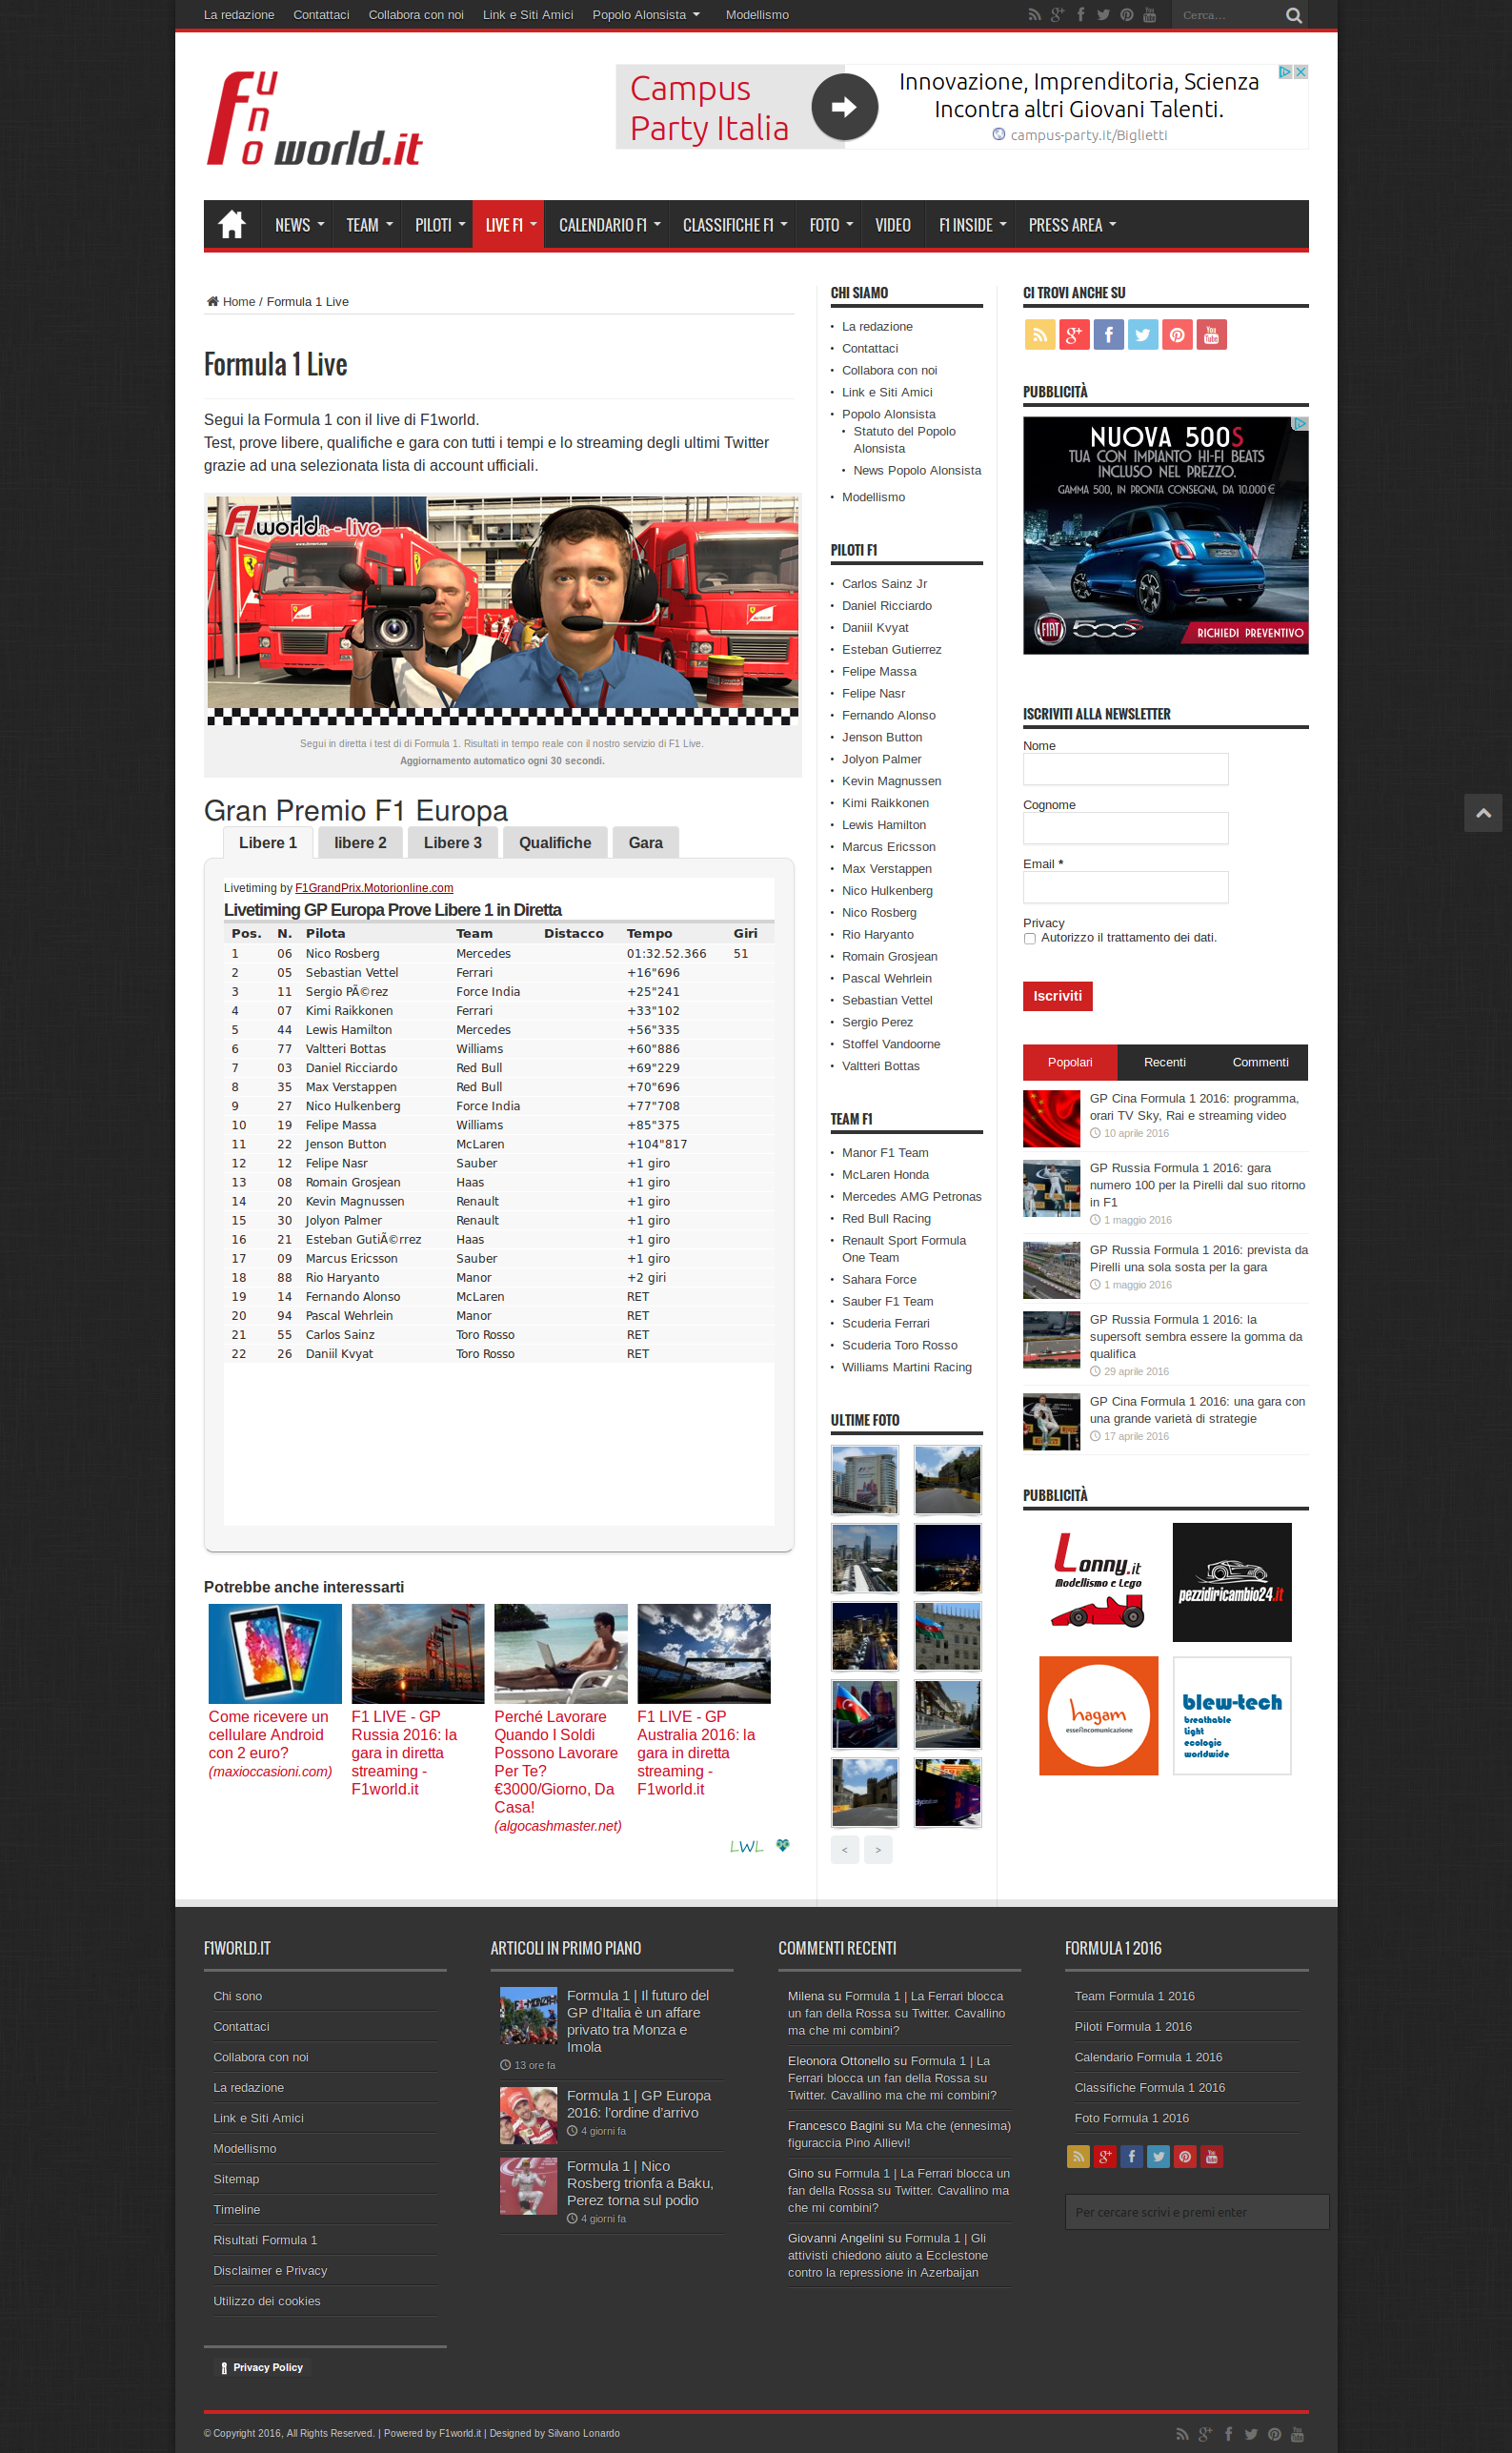
\includegraphics[height=18cm, width=10cm]{res/img/Formula1Live_Full}
  \caption{\textit{Screenshot} della sezione ``Formula1 Live''}
\end{figure}

Questa pagina presenta diversi difetti a livello di usabilità.
Innanzitutto è presente un'immagine (che potrebbe essere a mio avviso
migliorabile) all'inizio, che aumenta il numero di scroll. Inoltre
questa pagina non risulta utile ai fini del contenuto stesso, occupando solo
spazio.

Scendendo nella pagina possiamo trovare una tabella suddivisa per
schede. Per ogni scheda è presente la classifica della sessione, che si aggiorna
in tempo reale. Questa tabella presenta problemi relativi ai caratteri
accentati, che non vengono visualizzati correttamente e anche problemi relativi
alla visualizzazione della tabella stessa, che presenta uno spazio bianco
vuoto senza una apparente motivazione.

Riguardo al contenuto, è possibile vedere come la scheda ``Prove libere''
sia uguale alle informazioni presenti nella scheda ``Gara''. Questo problema
causa all'utente disorientamento, in quanto dovrebbe aspettarsi di vedere
informazioni diverse sui tempi in base alla sessione selezionata.

\begin{figure}[H]
    \centering
    \begin{subfigure}[b]{0.45\textwidth}
        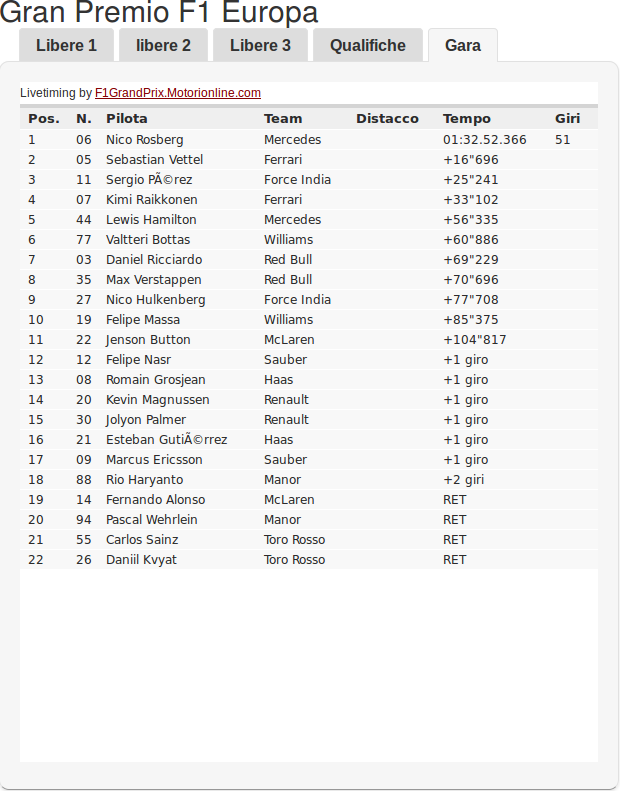
\includegraphics[scale=0.25]{res/img/dettagli/tableScoreR}
        \caption{Tempi presenti nella sezione ``Gara''}
    \end{subfigure}
    ~
    \begin{subfigure}[b]{0.45\textwidth}
        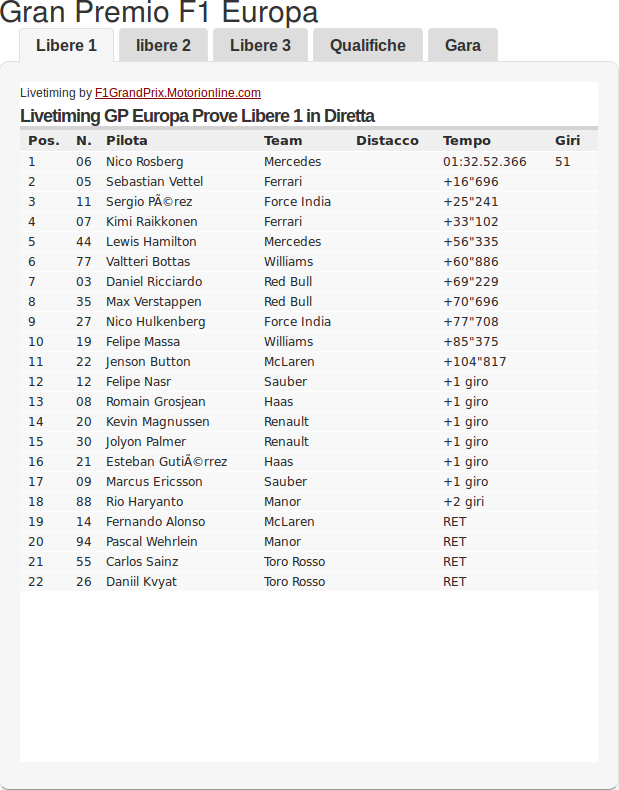
\includegraphics[scale=0.25]{res/img/dettagli/tableScoreFP1}
        \caption{Tempi presenti nella sezione ``Prove libere''}
    \end{subfigure}
    \caption{Confronto dei dati tra le tabelle}
\end{figure}

All'inizio della pagina viene annunciata la presenza di uno stream di
\textit{twitt} dagli account ufficiali de team. Questo stream non è però
presente, causando quindi stress e delusione all'utente, che si ritrova alla
ricerca di informazioni che non sono presenti.

La pagina presenta un difetto globale: ogni 30 secondi viene eseguito un
\textit{refresh} automatico, senza possibilità di annullarlo. Questo genera
molta frustrazione all'utente, che si vede ogni 30 secondi ricaricarsi la pagina.
Dovrebbe essere data la possibilità all'utente di decidere se si vuole o meno
il \textit{refresh} automatico, magari fornendo un apposito bottone e non
ricaricando tutta la pagina, ma solo le informazioni della tabella.

Finito il contenuto è presente una sezione di articoli a riguardo, in cui sono
presenti annunci pubblicitari.
